\chapter{\IfLanguageName{dutch}{Stand van zaken}{State of the art}}%
\label{ch:stand-van-zaken}

% Tip: Begin elk hoofdstuk met een paragraaf inleiding die beschrijft hoe
% dit hoofdstuk past binnen het geheel van de bachelorproef. Geef in het
% bijzonder aan wat de link is met het vorige en volgende hoofdstuk.

% Pas na deze inleidende paragraaf komt de eerste sectie hoofding.

%Dit hoofdstuk bevat je literatuurstudie. De inhoud gaat verder op de inleiding, maar zal het onderwerp van de bachelorproef *diepgaand* uitspitten. De bedoeling is dat de lezer na lezing van dit hoofdstuk helemaal op de hoogte is van de huidige stand van zaken (state-of-the-art) in het onderzoeksdomein. Iemand die niet vertrouwd is met het onderwerp, weet nu voldoende om de rest van het verhaal te kunnen volgen, zonder dat die er nog andere informatie moet over opzoeken \autocite{Pollefliet2011}.

%Je verwijst bij elke bewering die je doet, vakterm die je introduceert, enz.\ naar je bronnen. In \LaTeX{} kan dat met het commando \texttt{$\backslash${textcite\{\}}} of \texttt{$\backslash${autocite\{\}}}. Als argument van het commando geef je de ``sleutel'' van een ``record'' in een bibliografische databank in het Bib\LaTeX{}-formaat (een tekstbestand). Als je expliciet naar de auteur verwijst in de zin, gebruik je \texttt{$\backslash${}textcite\{\}}.
%Soms wil je de auteur niet expliciet vernoemen, dan gebruik je \texttt{$\backslash${}autocite\{\}}. In de volgende paragraaf een voorbeeld van elk.

%\textcite{Knuth1998} schreef een van de standaardwerken over sorteer- en zoekalgoritmen. Experten zijn het erover eens dat cloud computing een interessante opportuniteit vormen, zowel voor gebruikers als voor dienstverleners op vlak van informatietechnologie~\autocite{Creeger2009}.

%\lipsum[7-20]

Met dit onderzoek is het de bedoeling tot een goede oplossing te komen om de installatie van de nodige software voor de oefeningen van het vak Big Data Processing aan HoGENT zoveel mogelijk te automatiseren.
Meer concreet worden tijdens deze oefeningen de applicaties Hadoop, Spark en Kafka gebruikt. Momenteel wordt deze software geïnstalleerd tijdens de les zelf en dat is verlies van tijd die nuttiger zou zijn voor het gebruik van de applicaties in plaats van voor de installatie ervan. 
\newline
\newline
Een extra doelstelling is om deze applicaties ook tijdens de examens te kunnen gebruiken op een centrale installatie van HoGENT, met inachtname van veiligheid en stabiliteit.
\newline
\newline
Voor het gebruik van deze applicaties zijn typisch telkens 2 ervan nodig, bijvoorbeeld Hadoop in combinatie met Spark of Spark in combinatie met Kafka. Meer hierover verder in dit hoofdstuk.
\newline
\newline
Gezien het doel van deze studie, te komen tot een installatie ter ondersteuning van de oefeningen, zal het onderzoek zich vooral focussen op de functionaliteiten die tijdens de les gebruikt worden en op aspecten van belang voor de installatie, niet op de volledige werking van de verschillende softwares.
\newline
\newline

\section{Containertechnologie}
Container technology is a lightweight, executable unit of software that packs up application code and dependencies such as binary code, libraries, and configuration files for easy deployment across different computing environments \autocite{Solarwinds2023}.

\subsubsection{Container}
Containers are an abstraction at the app layer that packages code and dependencies together. Multiple containers can run on the same machine and share the OS kernel with other containers, each running as isolated processes in user space. Containers take up less space than VMs (container images are typically tens of MBs in size), can handle more applications and require fewer VMs and Operating systems.\autocite{Docker2023a}
\newline
\newline
Met containertechnologie wordt de basis van het Operating Systeem gedeeld met de verschillende containers in tegenstelling tot Virtual Machines, die kunnen aanzien worden als een voorganger van containers, waar een volledige `virtuele computer` telkens wordt gebruikt, inclusief het Operating Systeem. Hierdoor zijn containers veel kleiner, zowel wat disk space als geheugen betreft.
\newline
\newline
De meest gebruikte containersoftware is Docker en rekening houdende met andere zaken zoals
\begin{itemize}
    \item De VIC omgeving: Docker containers worden als de-facto standaard ondersteund op vSphere e winnen aan belang ten opzichte van virtuele machines
    \item De Big Data applicaties: deze zijn allemaal beschikbaar als Docker Image
\end{itemize}
is de keuze genomen om te werken met Docker containers.

\subsection{Docker}
Docker is a software platform that allows you to build, test, and deploy applications quickly. Docker packages software into standardized units called containers that have everything the software needs to run including libraries, system tools, code, and runtime. Using Docker, you can quickly deploy and scale applications into any environment and know your code will run. \autocite{AwsAmazon2023}
\newline
\newline
Een Docker container wordt gestart op basis van een Docker image, dit bevat alle nodige software en configuratie om een oplossing te kunnen draaien, soms zitten er ook al een deel voorgedefinieerde gegevens in. De container starten betekent het starten van de software in de image, typisch een startup script dat deel uitmaakt van de image.

\subsubsection{Image}
A Docker image is a lightweight, standalone, executable package of software that includes everything needed to run an application: code, runtime, system tools, system libraries and settings.\autocite{Docker2023a}
\newline
\newline
Docker images gebruiken een `parent` image, bijvoorbeeld een basis Linux container image, waaraan dan via commandos in de Dockerfile (een definitie tekst file) software wordt toegevoegd. De nieuwe image die op die manier wordt gemaakt verwijst naar de parent image maar bevat deze niet. Er wordt een `laag` aangemaakt die dan samen met de parent image kan uitgevoerd worden. Samen vormen ze de nieuwe image.
Deze kan op zijn beurt gebruikt worden als parent voor een andere image, die dan al uit 3 image lagen zal bestaan. Dit vormt een besparing op disk space en netwerk communicatie, want de images worden typisch centraal opgeslagen op DockerHub zodat ze door anderen kunnen gebruikt worden.
Merk op dat dit betekent dat de inhoud van deze image layers niet kan gewijzigd worden, anders zou de container met Image A gebaseerd op Image X de inhoud wijzigen van Image B ook gebaseerd op Image X. 

\subsection{Volume}
Om de container dus toe te laten gegevens te bewaren introduceert Docker het concept van een volume. Dit is een opslagplaats waarvan de container kan gebruik maken, maar een volume maakt deel uit van de omgeving waar de container draait, bestaat dus buiten de container en blijft ook bestaan als de container is gestopt. Bijvoorbeeld voor een database container worden de databases zelf in een volume bewaart anders zou alles verloren gaan eens de container wordt gestopt.

Volumes are the preferred mechanism for persisting data generated by and used by Docker containers.
The data is kept somewhere on storage attached to the host - often the local filesystem. The volume itself has a lifecycle that's longer than the container's, allowing it to persist until no longer needed. Volumes can be shared between containers. \autocite{Javatpoint2023}
\newline
\newline
Docker containers are used to run applications in an isolated environment. By default, all the changes inside the container are lost when the container stops. If we want to keep data between runs, Docker volumes and bind mounts can help. \autocite{Frieze2022}
\newline
\newline
Het is hierbij ook good practice/standaard om per image/container maar 1 applicatie te installeren en draaien. Dat maakt het Docker image telkens gelinkt aan 1 oplossing, de meeste uitgevers van software stellen die ook ter beschikking als image op DockerHub, sommige software wordt door derden toegevoegd.
\newline
\newline
Dus wat we zeker al nodig hebben voor onze oplossing zijn 3 Docker images, 1 voor elke applicatie: Hadoop, Spark en Kafka. Voor alle drie is er een image beschikbaar op DockerHub, die vormen een goede start waaraan we dan zaken kunnen toevoegen indien nodig.
\newline
\newline
De volgende stap is het automatiseren van het gecombineerd opstarten van applicaties die samenwerken, bijvoorbeeld Hadoop en Spark. Hiervoor kijken we naar een tool `docker-compose` genaamd.

\subsection{Docker-compose}
Docker Compose is a tool that was developed to help define and share multi-container applications. With Compose, we can create a YAML file to define the services and with a single command, can spin everything up or tear it all down. \autocite{Docker2023}
\newline
\newline
In een Docker Compose file worden de verschillende services die samenwerken gedefiniëerd. Elke service is gebaseerd op een Docker image, per service kunnen we volumes toevoegen, netwerken opzetten die toelaten aan de verschillende containers om te communiceren, dependencies tussen services (welke eerst moet gestart worden), parameters die bepalen wanneer een container moet herstart worden, enz.
\newline
\newline
Met 1 docker compose commando wordt de combinatie van services dan opgestart.
\newline
\newline
Onze oplossing zou dus kunnen bestaan uit meerdere docker-compose files, telkens voor een combinatie van de Big Data applicaties. Dit gaan we moeten uitzoeken.
\newline
\newline

\subsection{Cluster}
Een cluster is een groep van computers of nodes die samenwerken en zich naar de gebruiker toe als 1 enkel systeem gedragen, waarbij het werk wordt verdeeld over de verschillende nodes. Dit laat toe om extra nodes op te starten bij meer belasting en terug af te sluiten om resources te sparen (Scalability), nodes te herstarten zonder dat de gebruiker er iets van merkt (Stability; Availability).\textcite{Nordhoff2020}
\newline
\newline
Bij een Docker cluster, ook Docker swarm genoemd, worden de containers verdeeld over verschillende nodes door cluster management van de Docker engine zelf. Een swarm bestaat uit meerdere Docker hosts, waarop zowel een manager als een worker kunnen draaien, en waarbij de managers de gewenste containers verdelen over de worker nodes, rekening houdende met specificaties zoals welke opslag resources, netwerken en aantal instanties gewenst zijn. De Docker engine zorgt voor de connectiviteit tussen de containers, gelijkaardig aan ``bridge'' netwerken die containers binnen één enkele computer verbinden.\textcite{BMitch2019}
TODO https://docs.docker.com/engine/swarm/key-concepts/ en verwijder BMitch2019
\newline
\newline
Docker Swarm is een mogelijkheid voor de installatie en het beheer van Big Data oplossingen.
\newline
\newline


\subsection{Kubernetes}
Kubernetes, of K8s, is een open-source container oplossing ontworpen door Google. Het wordt gebruikt om groepen of clusters van applicaties binnen containers te beheren. Dit noemen we in de IT wereld ‘orkestratie’. (https://nl.wikipedia.org/wiki/Orkestratie_(informatica))
\newline
Kubernetes start en monitort containers, start extra containers indien nodig om de belasting aan te kunnen, en stopt en herstart automatisch containers die niet langer reageren.\textcite{Guthrie2022}
\newline
\newline
De laatste jaren worden containers meer en meer gebruikt en Kubernetes is zowat de standaard geworden voor bedrijven om hun containers te beheren en automatiseren.
(TODO) https://www.linkedin.com/pulse/kubernetes-the-de-facto-standard-deploy-operate-containerized-/
\newline
\newline
Een belangrijk onderdeel van Kubernetes is de netwerk communicatie. Er zijn meerdere types communicatie, namelijk die tussen containers in eenzelfde pod (eenvoudig gebruik van localhost), die tussen Pods onderling, en die van de buitenwereld naar een service, deze laatste is een manier om toegang te verlenen tot een applikatie die binnen de cluster op meerdere Pods draait.

TODO https://kubernetes.io/docs/concepts/cluster-administration/networking/
TODO https://kubernetes.io/docs/concepts/services-networking/service/
\newline
\newline
We gaan dus zeker ook naar Kubernetes kijken en onderzoeken of het nuttig kan zijn bij het opzetten van onze oplossing.

\section{Hadoop}
Eerste enkele woordjes uitleg over de werking van Hadoop.
\newline
\newline
De Apache Hadoop oplossing is een raamwerk dat toelaat om grote sets van gegevens gedistribueerd te verwerken, waarbij die verdeling over clusters van computers toeganlijk ik via eenvoudige programmeermodellen, o.a. het gedistribueerde filesysteem HDFS.
\newline
Hadoop is ontworpen om als cluster gebruikt te worden, met fout detectie en afhandeling ervan, en kan gaan tot duizenden machines, elk met lokale verwerking en opslag. \textcite{ASF2022}

\subsection{Hadoop Distributed File System}
The Hadoop Distributed File System (HDFS) is a distributed file system designed to run on commodity hardware. It has many similarities with existing distributed file systems.
However, the differences from other distributed file systems are significant. HDFS is highly fault-tolerant and is designed to be deployed on low-cost hardware. HDFS provides high throughput access to application data and is suitable for applications that have large data sets.\autocite{Borthakur2007a}
\newline
\newline
Omn de data te verdelen over alle nodes die deelnemen aan de Hadoop cluster wordt HDFS gebruikt, dit heeft een master/slave architectuur en laat toe om gegevens op te slaan in files die verdeeld worden over de cluster. Een cluster bestaat uit 1 master, de namenode en meerdere slaves, de datanodes. Een 2e namenode wordt gebruikt als 
\newline
De namenode houdt bij in welke datanodes de data zich bevindt. Meerdere copies van de data worden gerepliceerd over de verschillende datanodes zodat er geen data verloren gaat bij uitvallen van een datanode.

\subsection{MapReduce}
MapReduce is a programming model or pattern within the Hadoop framework that is used to access big data stored in the Hadoop File System (HDFS). It is a core component, integral to the functioning of the Hadoop framework.
MapReduce facilitates concurrent processing by splitting petabytes of data into smaller chunks, and processing them in parallel on Hadoop commodity servers. In the end, it aggregates all the data from multiple servers to return a consolidated output back to the application.\autocite{Talend2023}
\newline
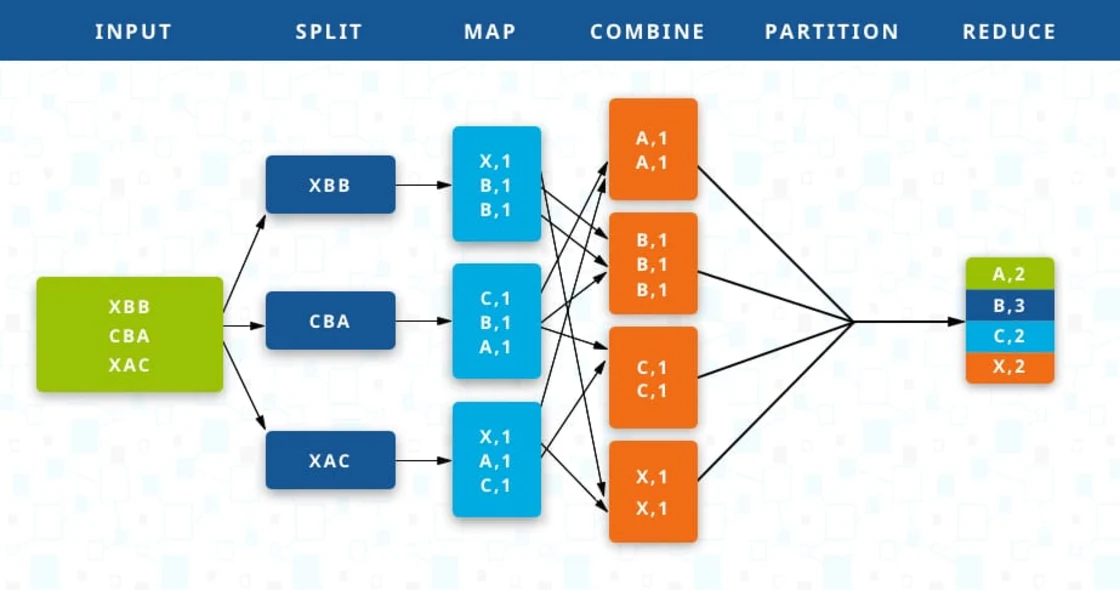
\includegraphics[scale=0.4]{mapreduce.jpg}
\newline
\newline
Hadoop wordt o.a. alleenstaand gebruikt tijdens de oefeningen Big Data Processing, daarvoor kunnen we bestaande Docker Compose files gebruiken die de verschillende services bevatten nodig om een Master of Slave te starten.
In de eenvoudigste vorm is er 1 docker compose file die alle services opstart om te kunnen werken met 1 master en 1 slave.
\newline
\newline
Elke service (namenode, datanode, resourcemanager) is een specifiek Docker image, ook beschikbaar op DockerHub. Er zijn voorbeelden te vinden van de Docker scripts die gebruikt werden om dit soort images te bouwen. Typisch is er een basis Hadoop images dat het volledige framework bevat, en worden daar aparte images vanaf geleid die telkens maar 1 specifiek process (namenode, datanode, ...) van Hadoop opstarten.
Door op die manier met aparte images te werken kan het beheer van de cluster buiten Hadoop worden gedaan, typisch in Kubernetes, zie verder.
\newline
\newline
In de volgende sectie gaan we Apache Spark bekijken, welke functionaliteit dit toevoegt aan Hadoop en hoe we dit kunnen integreren in Docker Compose.

\section{Spark}
Apache Spark is an open-source, distributed processing system used for big data workloads. It utilizes in-memory caching, and optimized query execution for fast analytic queries against data of any size.
Spark was designed for fast, interactive computation that runs in memory, enabling machine learning to run quickly. The algorithms include the ability to do classification, regression, clustering, collaborative filtering, and pattern mining.\autocite{AwsAmazon2023a}
\newline
\newline
Apache Spark is net als Hadoop een data processing engine voor Big Data. Spark verdeelt ook de taken en de gegevens over verschillende nodes, voor een aantal gevallen zal het sneller zijn dan Hadoop omdat het gebruik maakt van RAM geheugen in plaats van een bestandssysteem.
De data in Spark word verdeeld over een cluster opgeslagen, in eerdere versies in RDD (Resilient Distributed Dataset) zijnde een set van Java of Scala data objecten. In nieuwere versies van Spark wordt DataFrame gebruikt, waarbij de gegegvens gestructureerd worden in kolommen, gelijkaardig aan een tabel in een relationele databank.
TODO https://data-flair.training/blogs/apache-spark-rdd-vs-dataframe-vs-dataset/
\newline
\newline
Spark bevat meerder componenten om aan data verwerking te doen: Spark SQL, Spark MLlib en Spark GraphX.

\subsection{Spark SQL}
Spark SQL is a Spark module for structured data processing. It provides a programming abstraction called DataFrames and can also act as distributed SQL query engine. It enables unmodified Hadoop Hive queries to run up to 100x faster on existing deployments and data.\autocite{databricks2023}

\subsection{Spark MLlib}
Machine learning has quickly emerged as a critical piece in mining Big Data for actionable insights. Built on top of Spark, MLlib is a scalable machine learning library that delivers both high-quality algorithms (e.g., multiple iterations to increase accuracy) and blazing speed (up to 100x faster than MapReduce).\autocite{databricks2023}

\subsection{Spark GraphX}
Apache Spark's API for graphs and graph-parallel computation.
GraphX is a graph computation engine built on top of Spark that enables users to interactively build, transform and reason about graph structured data at scale. It comes complete with a library of common algorithms.\autocite{databricks2023}
\newline
\newline
Deze componenten kunnen in Hadoop MapReduce vervangen, en indien de datasets volledig in het cache geheugen passen, kan dan tot 100x sneller zijn.


\subsection{Spark Streaming}
Many applications need the ability to process and analyze not only batch data, but also streams of new data in real-time. Running on top of Spark, Spark Streaming enables powerful interactive and analytical applications across both streaming and historical data, while inheriting Spark’s ease of use and fault tolerance characteristics. It readily integrates with a wide variety of popular data sources, including HDFS, Flume, Kafka, and Twitter.\autocite{databricks2023}
\newline
\newline
Het is dit laatste onderdeel, Spark Streaming, dat door Kafka (zie verder) kan worden gebruikt om data aan door te geven voor verdere verwerking.
\newline
\newline
Terugkomend op ons doel van Spark in Docker containers te draaien, er zijn Spark Docker images beschikbaar die toelaten zowel een Spark Master als Worker te starten.
\newline
\newline
Er zijn ook voorbeelden te vinden van discussies over mogelijke manieren om Hadoop en Spark te combineren in Docker Compose.


\section{Kafka}
Apache Kafka is a distributed data store optimized for ingesting and processing streaming data in real-time. Streaming data is data that is continuously generated by thousands of data sources, which typically send the data records in simultaneously. A streaming platform needs to handle this constant influx of data, and process the data sequentially and incrementally.
\autocite{AwsAmazon2023b}

\subsection{Broker}
A Kafka broker receives messages from producers and stores them on disk keyed by unique offset. A Kafka broker allows consumers to fetch messages by topic, partition and offset. Kafka brokers can create a Kafka cluster by sharing information between each other directly or indirectly using Zookeeper.\autocite{GitBook2023}

\subsection{Topic}
What are Apache Kafka Topics? Apache Kafka has a dedicated and fundamental unit for Event or Message organization, called Topics. In other words, Kafka Topics are Virtual Groups or Logs that hold messages and events in a logical order, allowing users to send and receive data between Kafka Servers with ease.\autocite{Ishwarya2022}

\subsection{Partitions}
What Is a Kafka Partition? In Apache Kafka, partitions are the main method of concurrency for topics. A topic, a dedicated location for events or messages, will be broken into multiple partitions among one or more Kafka brokers\autocite{Carder2022}
\newline
\newline
Er zijn Kafka Docker images beschikbaar en er zijn ook voorbeelden te vinden van discussies over mogelijke manieren om Kafka en Spark te combineren in Docker Compose.
\newline
\newline
In vorige versies van Kafka werd Zookeeper gebruikt voor opslag van metadata. In recente versies is dit vervangen door een intern systeem, wat beter is omdat gebruikers dan geen extra applicatie moeten leren opzetten en er worden ook minder resources gebruikt.

\section{Zookeeper}
ZooKeeper is a centralized service for maintaining configuration information, naming, providing distributed synchronization, and providing group services. All of these kinds of services are used in some form or another by distributed applications. Each time they are implemented there is a lot of work that goes into fixing the bugs and race conditions that are inevitable.\autocite{ASF2023}
\newline
\newline 
What is ZooKeeper in Apache Kafka?
Zookeeper is used for metadata management in the Kafka world. For example: Zookeeper keeps track of which brokers are part of the Kafka cluster. Zookeeper is used by Kafka brokers to determine which broker is the leader of a given partition and topic and perform leader elections. \autocite{Conduktor2023}
\newline
\newline
Afhankelijk van de versie van Kafka die we uiteindelijk zullen gebruiken zal Zookeeper wel of niet toegevoegd worden aan de Docker compose.
\newline
\newline
\newline
\newline
\newline
Hadoop, Spark en Kafka worden al samen gebruikt volgens \textcite{Holmes2012}:
'In this situation, you'd use Kafka to both land data on Hadoop and provide a feed into a real-time data-streaming system such as Storm or Spark Streaming, which you could then use to perform near-real-time computations.' en \textcite{Leang2019}:
'one of the more significant findings to emerge from this study is that the integration of the Hadoop system especially Apache Kafka and Apache Spark enhances the performance and accuracy of data storing, processing, and securing in the manufacturing environment.'
\newline
\newline
Er is informatie te vinden over het gebruik van Docker compose om verschillende combinaties van 2 van de 3 frameworks te installeren maar niks over alle 3 samen, zeker niet met de requirements die wij willen onderzoeken (een afzonderlijke scalable beveiligde `cluster` per student).



\section{Virtual IT Company(VIC)}
VIC is een ``bedrijf'' in HoGENT dat virtuele machines voorziet voor studenten, zodat bepaalde oplossingen niet op een eigen computer moet draaien, en op aanvraag maken ze de virtuele machine(s), er wordt een soort van contract afgesproken met machine specs en lifespan.
\newline
\newline
VIC gebruikt de oplossing van VMWare (vSphere, VMWare ESXi Hypervisor) voor het beheer van virtuele machines op de eigen hardware.
TODO

\subsection{Hypervisor}
A hypervisor, also known as a virtual machine monitor or VMM, is software that creates and runs virtual machines (VMs). A hypervisor allows one host computer to support multiple guest VMs by virtually sharing its resources, such as memory and processing.\autocite{VMware2023a}

\subsection{VMWare ESXi}
Discover a robust, bare-metal hypervisor that installs directly onto your physical server. With direct access to and control of underlying resources, VMware ESXi effectively partitions hardware to consolidate applications and cut costs. It’s the industry leader for efficient architecture, setting the standard for reliability, performance, and support.\autocite{VMware2023}

\subsection{vCenter}
vCenter Server is the centralized management utility for VMware, and is used to manage virtual machines, multiple ESXi hosts, and all dependent components from a single centralized location. VMware vMotion and svMotion require the use of vCenter and ESXi hosts.\autocite{Abbas2023}
\newline
\newline
Momenteel wordt er nog geen Kubernetes gebruikt in het VIC. Ook geen Docker containers, alles is gebaseerd op virtuele machines.
\newline
\newline
VMWare vSphere, dit is de set van VMWare Virtualization applicaties, ondersteunt intussen ook Kubernetes.
\newline
\newline
De volgende componenten zijn van belang om het gebruik van Kubernetes op VMware te begrijpen. De concepten van Kubernetes worden gelinkt aan VMWare concepten.

\subsection{Nodes}
There are two main node types in Kubernetes, a Master and Worker. A master node is a management node, what you would expect of vCenter Server. A worker node is what you would expect of an ESXi host, allowing you to run Pods.\autocite{VMware2019}

\subsection{Pod}
A Pod is a group of one or more containers. If we map this to a VMware Administrator construct think of Pods as an object similar to a virtual machine. Pods are managed by the Kubelet that runs on each node. Kubelet watches Podspecs assigned to it and handles all lifecycle by comparing actual Pod state to the desired state stored in the Podspec.\autocite{VMware2019}

\subsection{Namespace}
A Namespace is used as the unit of management in environments with many users across multiple teams or projects. Namespaces are a way to divide cluster resources and separate permissions between users. When a Namespace is created you assign CPU, Memory and Storage limits to restrict the amount of resources a workload can consume, not unlike a vSphere Resource Pool. Where Namespaces differ from Resource Pools is that they also incorporate controls such as security. For example, from a security perspective via Namespaces you can manage access controls by using edit or read-only groups. You also have the ability through security policies to limit ports, audit changes and force encryption of data. To encrypt all containers and/or VMs in a Namespace is done by setting one property rather than going to each VM and encrypting individually.\autocite{VMware2019}
\newline
\newline
Kubernetes wordt ondersteund om Developers te laten werken met gekende tools en begrippen zodat ze zich niet moeten verdiepen in VNWare vSphere.
\newline
\newline
To a developer, vSphere with Kubernetes looks and acts like a standard Kubernetes cluster. Their tools and processes work across implementations. They can use the Kubernetes “declarative syntax” to define what resources they need, such as storage, networking, and even relationships \& availability requirements. By using the industry-standard Kubernetes syntax they don’t need direct access to, or knowledge of, the vSphere APIs, clients, or infrastructure.\autocite{VMware2019}
\newline
\newline
Daarnaast worden Docker containers en Docker Compose ondersteund door VNWare vSphere, dus dit is ook nog een mogelijke oplossing zonder Kubernetes. 
\newline
\newline
\newline
Om te onderzoeken hoe aan de security en stability (isolatie van gebruikers) eisen kan worden voldaan, gaan we o.a. Namespaces verder bestuderen. Daarnaast gaan we ook bekijken in hoeverre het gebruik van een reverse proxy (bv. Nginx) de toegang tot een Pod kan afschermen om op die manier maar 1 student per Pod toe te laten te connecteren op de consoles van Hadoop, Spark en Kafka.
\newline
\newline
Voor de configuratie van Nginx basic authentication en users kijken we o.a. naar Kubernetes ConfigMap.

\subsection{ConfigMap}
A ConfigMap is an API object used to store non-confidential data in key-value pairs. Pods can consume ConfigMaps as environment variables, command-line arguments, or as configuration files in a volume.
A ConfigMap allows you to decouple environment-specific configuration from your container images, so that your applications are easily portable.\autocite{Kubernetes2023}
